\begin{comment}
\begin{figure}[H]
\centering
	\begin{tikzpicture}
		\begin{axis}[
		axis lines = middle,
		xlabel = $x$,
		ylabel = {$f(x)$}]
        \addplot[
        domain=-3:3,
        samples=10,
        color=blue,
        ]{3*x+2};
        \addlegendentry{$f(x)=3x+2$}
		\end{axis}
	\end{tikzpicture}
\end{figure}
\end{comment}


\begin{figure}[H]
\centering
	\begin{subfigure}[b]{0.45\textwidth}
	\centering
    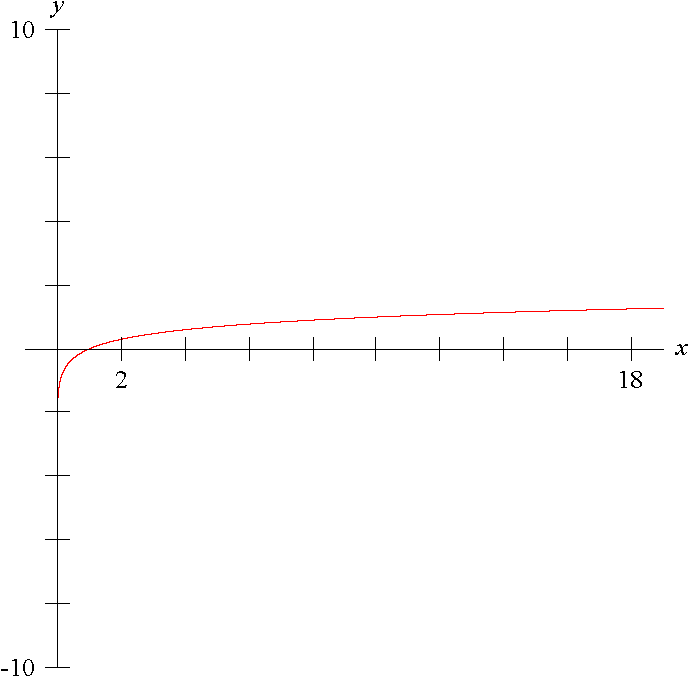
\includegraphics[width=1\textwidth]{calculo/images/logaritmo_normal}
	\caption{$f(x)=\log_{10}(x)$}
	\end{subfigure}
	\quad
	\begin{subfigure}[b]{0.45\textwidth}
	\centering
    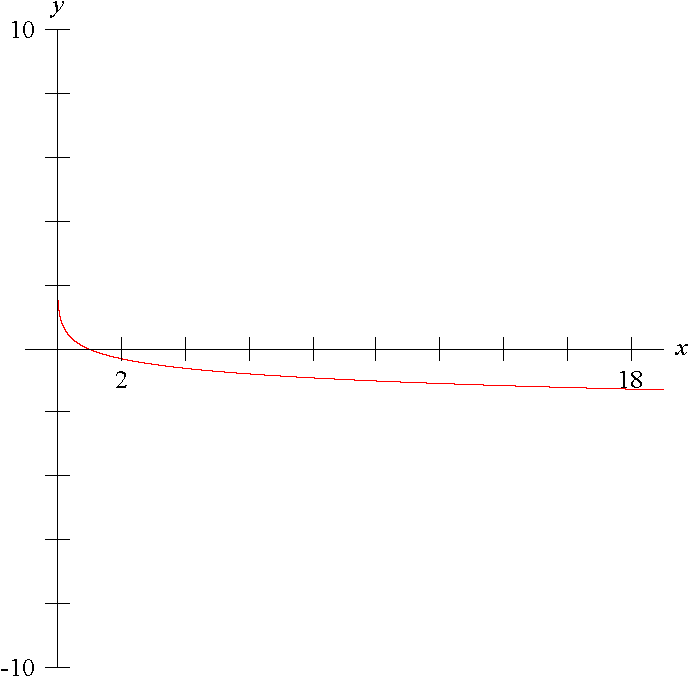
\includegraphics[width=1\textwidth]{calculo/images/logaritmo}
	\caption{$f(x)=\log_{\frac{1}{10}(x)}$}
	\end{subfigure}
\caption{Função Logarítmica}
\end{figure}


\begin{figure}[H] 
\label{exp1}
\centering
	\begin{tikzpicture}
		\begin{axis}[
		axis lines = middle,
        xlabel = $x$,
        ylabel = $y$]
        \addplot[
        domain = -3:3,
        samples = 100,
        ]{2^x};
        \addlegendentry{$f(x)=2^x$}
		\end{axis}\
	\end{tikzpicture}
\end{figure}

\begin{figure}[H] 
\label{exp2}
\centering
	\begin{tikzpicture}
		\begin{axis}[
		axis lines = middle,
        xlabel = $x$,
        ylabel = $y$]
        \addplot[
        domain = -3:3,
        samples = 100,
        ]{(0.5)^x};
        \addlegendentry{$f(x)=\left(\frac{1}{2}\right)^x$}
		\end{axis}\
	\end{tikzpicture}
\end{figure}

\begin{figure}[H] 
\label{log}
\centering
	\begin{tikzpicture}
		\begin{axis}[
		axis lines = middle,
        xlabel = $x$,
        ylabel = $y$]
        \addplot[
        domain = 0:7,
        samples = 100,
        ]{log10(x)};
        \addlegendentry{$f(x)=\log_{10} x$}
		\end{axis}\
	\end{tikzpicture}
\end{figure}

\begin{figure}[H] 
\label{log2}
\centering
	\begin{tikzpicture}
		\begin{axis}[
		axis lines = middle,
        xlabel = $x$,
        ylabel = $y$]
        \addplot[
        domain = 0:7,
        samples = 100,
        ]{-log10(x)};
        \addlegendentry{$f(x)=\log_{\frac{1}{10}} x$}
		\end{axis}\
	\end{tikzpicture}
\end{figure}

\begin{figure}[H] 
\label{seno}
\centering
	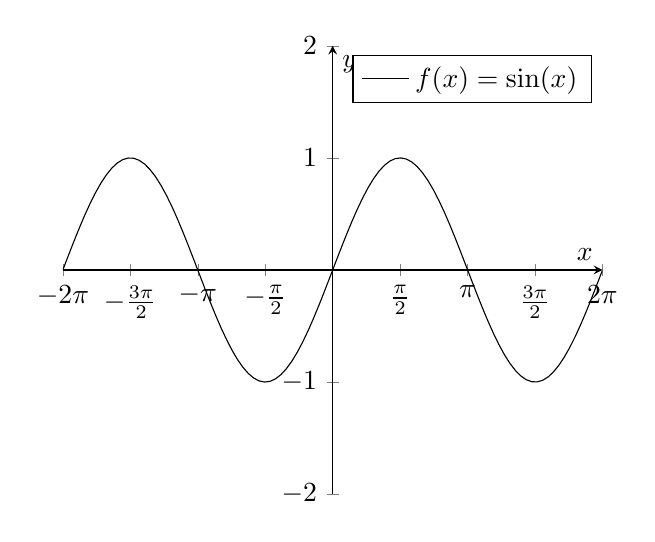
\begin{tikzpicture}
		\begin{axis}[
		axis lines = middle,
        xtick = {-6.28,-4.71,-3.14,-1.57,0,1.57,3.14,4.71,6.28},
        xticklabels ={$-2\pi$,$-\frac{3\pi}{2}$,$-\pi$,$-\frac{\pi}{2}$,$0$,$\frac{\pi}{2}$,$\pi$,$\frac{3\pi}{2}$,$2\pi$},
        xlabel = $x$,
        ylabel = $y$,
        ymin = -2,
        ymax = 2]
        \addplot[
        domain = -2*pi:2*pi,
        samples = 100,
        ]{sin(deg(x))};
        \addlegendentry{$f(x)=\sin(x)$}
		\end{axis}
	\end{tikzpicture}
\end{figure}
%como deixar a escala boa?
\begin{figure}[H] 
\label{cosseno}
\centering
	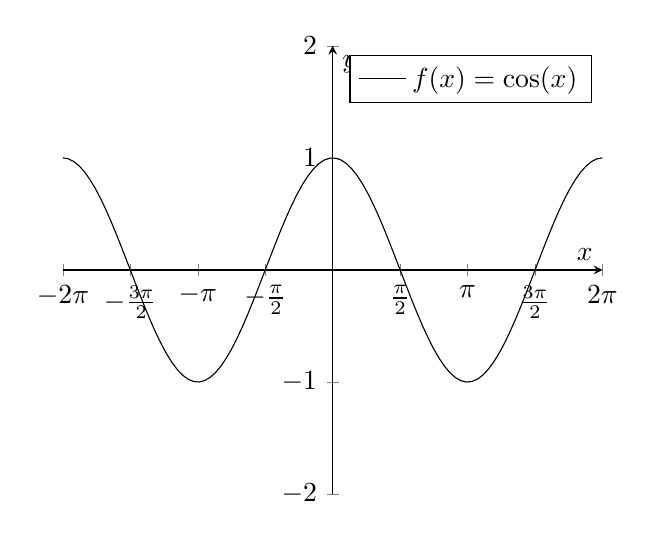
\begin{tikzpicture}
		\begin{axis}[
		axis lines = middle,
        xtick = {-6.28,-4.71,-3.14,-1.57,0,1.57,3.14,4.71,6.28},
        xticklabels ={$-2\pi$,$-\frac{3\pi}{2}$,$-\pi$,$-\frac{\pi}{2}$,$0$,$\frac{\pi}{2}$,$\pi$,$\frac{3\pi}{2}$,$2\pi$},
        xlabel = $x$,
        ylabel = $y$,
        ymin = -2,
        ymax = 2]
        \addplot[
        domain = -2*pi:2*pi,
        samples = 100,
        ]{cos(deg(x))};
        \addlegendentry{$f(x)=\cos(x)$}
		\end{axis}\
	\end{tikzpicture}
\end{figure}

\begin{figure}[H] 
\label{tangente}
\centering
	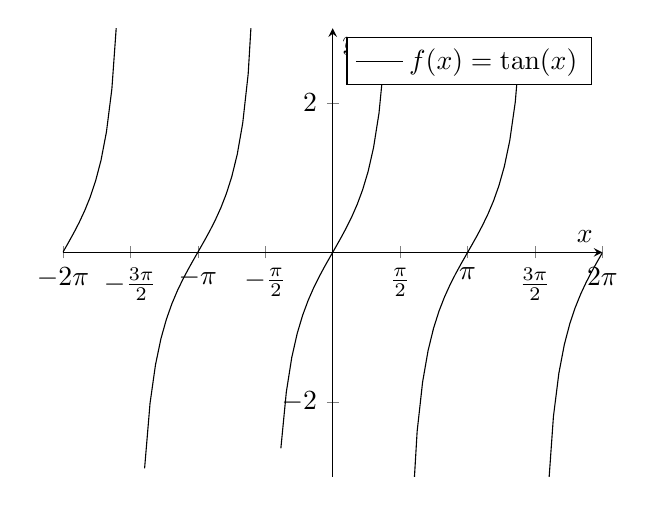
\begin{tikzpicture}
		\begin{axis}[
		axis lines = middle,
        xtick = {-6.28,-4.71,-3.14,-1.57,0,1.57,3.14,4.71,6.28},
        xticklabels ={$-2\pi$,$-\frac{3\pi}{2}$,$-\pi$,$-\frac{\pi}{2}$,$0$,$\frac{\pi}{2}$,$\pi$,$\frac{3\pi}{2}$,$2\pi$},
        xlabel = $x$,
        ylabel = $y$,
        ymin = -3,
        ymax = 3,
        restrict y to domain= -4:4]
        \addplot[
        domain = -2*pi:2*pi,
        samples = 100,
        ]{tan(deg(x))};
        \addlegendentry{$f(x)=\tan(x)$}
		\end{axis}
	\end{tikzpicture}
\end{figure}